\documentclass{beamer}

\usepackage[utf8]{inputenc}
\usepackage[T1]{fontenc}

\usepackage[english]{babel}
\usepackage{amsmath}
\usepackage{cleveref}
\usepackage{amssymb}
\usepackage{mathtools}

%%Numbers, expectation
\newcommand{\N}{\mathbb{N}}
\newcommand{\E}{\mathbb{E}}
\renewcommand{\P}{\mathbb{P}}
\newcommand{\Var}{\mathbb{V}}
\newcommand{\R}{\mathbb{R}}
\newcommand{\D}{\mathcal{D}}
\newcommand{\B}{\mathcal{B}}
\newcommand{\Dh}{\D_h}
\renewcommand{\phi}{\varphi}
\newcommand*\diff{\mathop{}\!\mathrm{d}} % integral

%% mathoperator
\DeclareMathOperator*{\argmax}{arg\,max}
\DeclareMathOperator*{\argmin}{arg\,min}
\DeclareMathOperator*{\dom}{dom}
\DeclareMathOperator*{\sign}{sign}
\DeclareMathOperator*{\diag}{diag}

\DeclareMathOperator*{\Cov}{Cov}
\DeclareMathOperator*{\Cor}{Corr}
\DeclareMathOperator*{\Id}{Id}

%proximal operator
\newcommand{\prox}[3][]{\operatorname{prox}^{#1}_{#2}\left(#3 \right)}

\usepackage{xcolor}

%% sort citations by increasing number
\usepackage[sort,nocompress]{cite}

\usepackage{graphicx}% http://ctan.org/pkg/graphicx
\graphicspath{{../figures/}{../../figures}{../../memes}} %Setting the graphicspath
\usepackage{caption,subcaption}

\usepackage{tikz}
\usepackage{pgfplots}
\usetikzlibrary{backgrounds}
\usetikzlibrary{intersections}
\usepgfplotslibrary{fillbetween}

% \usepackage[right]{showlabels}


%%
\theoremstyle{plain}
\newtheorem{prop}{Proposition}[section]
\newtheorem{algo}{Algorithm}[section]
\newtheorem{assumption}{Assumption}
\theoremstyle{remark}
\newtheorem{remark}{Remark}[section]

% cref
\crefname{assumption}{Assumption}{Assumptions}
\crefname{equation}{}{}

\usepackage{autonum}

\usepackage{bm} %% bold math symbols

\usepackage{bbm} %% for \mathbbm{1}


% algorithmic environment
\usepackage{algorithm}
\usepackage[noend]{algpseudocode}

% for some reason this was required on one void linux installation (but not the other)
\usepackage{sansmathaccent}
\pdfmapfile{+sansmathaccent.map}

\author{Axel Böhm}

% shows which section we're in
\usetheme{Darmstadt}

% page number
\setbeamertemplate{footline}[frame number]
\setbeamercolor{page number in head/foot}{fg=gray}


% display things like onslide or visible already before but grayed out
\setbeamercovered{transparent}

% set the itemize item symbol as a diamond
\setbeamertemplate{itemize item}{$\diamond$}
% set the itemize subitem symbol as a triangle
\setbeamertemplate{itemize subitem}{$\blacktriangleright$}

% set the enumerate item symbol as a roman numbers
\setbeamertemplate{enumerate item}{(\roman{enumi})}


\author{Axel Böhm}

% shows which section we're in
\usetheme{Darmstadt}

% page number
\setbeamertemplate{footline}[frame number]
\setbeamercolor{page number in head/foot}{fg=gray}


% display things like onslide or visible already before but grayed out
\setbeamercovered{transparent}

% set the itemize item symbol as a diamond
\setbeamertemplate{itemize item}{$\diamond$}
% set the itemize subitem symbol as a triangle
\setbeamertemplate{itemize subitem}{$\blacktriangleright$}

% set the enumerate item symbol as a roman numbers
\setbeamertemplate{enumerate item}{(\roman{enumi})}


\title{Optimization for Data Science}

\begin{document}
\maketitle
\frame{\tableofcontents}

\begin{frame}
  \frametitle{Course organization}
  \begin{itemize}
    \item Lectures (contribution counts)
    \item hands on sessions on some Thursdays
    \item a small weekly problem set
    \item Project (prices for most creative, best presentation, cleanest code, etc.)
    \item oral exam
  \end{itemize}

  Find everything on github (please contribute with pull requests: typos, etc.)

  \begin{itemize}
    \item Quick introductory round?
  \end{itemize}

\end{frame}



\section{Introduction}

\begin{frame}
  \frametitle{What is Optimization}

  \begin{center}
    \textit{Given a function $f$ which represents some cost/regret/loss (or gain/profit/utility) we aim to find the argument/decision associated with the smallest cost (or largest profit).}
  \end{center}

  \begin{equation}
    \min_{x\in C } \, f(x)
  \end{equation}

  \begin{itemize}
    \item variables, parameters, candidate solutions $x$
    \item objective function $f$ (typically real-valued)
    \item typically: technical assumptions on $f$
    \item constrained set $C \subset \R^d$
    \item convexity / differentiability
  \end{itemize}
\end{frame}


\begin{frame}
  \frametitle{Applications of optimization}

  \begin{itemize}
    \item Economics
          \begin{itemize}
            \item Microeconomics: Agents maximizing utility
            \item Game theory and equilibria
          \end{itemize}
    \item Statistics
          \begin{itemize}
            \item maximum likelihood
          \end{itemize}
    \item Physics
          \begin{itemize}
            \item soap bubble is a sphere because it minimizes surface tension
          \end{itemize}
    \item Chemistry
          \begin{itemize}
            \item Protein folding
          \end{itemize}
    \item Inverse problems
          \begin{itemize}
            \item imaging, denoising, deblurring
          \end{itemize}
  \end{itemize}

\end{frame}

\begin{frame}
  \frametitle{Optimization for ML}
  \begin{minipage}{0.5\textwidth}
    \begin{equation}
      \min_{\beta_1, \beta_0} \sum_{i=1}^{n} {( \beta_1 x_i + \beta_0 - y_i)}^2
    \end{equation}
    For data points $(x_i, y_i)$.
  \end{minipage}
  \hfill
  \begin{minipage}{0.45\textwidth}
    \begin{figure}[ht]
      \centering
      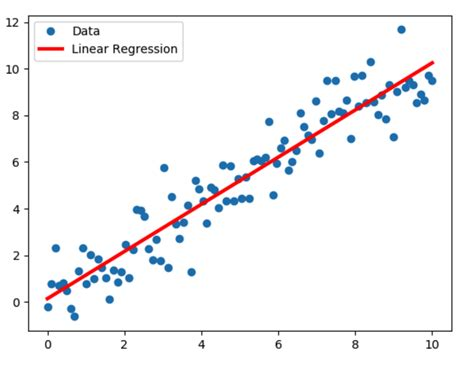
\includegraphics[width=\textwidth,height=\textheight,keepaspectratio]{linear_regression.jpg}
      % \caption{\label{fig:label} }
    \end{figure}
  \end{minipage}

  \begin{itemize}
    \item Loss functions express the discrepancy between the predictions of the model being trained and the actual problem instances
  \end{itemize}
\end{frame}

\begin{frame}
  \frametitle{Optimization for ML}
  \begin{itemize}
    \item \textcolor{blue}{Mathematical modeling}
          \begin{itemize}
            \item defining \& modeling the problem
            \item finding a good metric / what is success
            \item accuracy vs.\ solvability trade-off
          \end{itemize}
    \item \textcolor{blue}{Computational optimization}
         \begin{itemize}
           \item running an (appropriate) optimization algorithm
         \end{itemize}
    \item theory vs. practice
          \begin{itemize}
            \item libraries available, but algorithms treated as ``black box'' by practitioners
            \item we will try and understand why and how they work
          \end{itemize}
  \end{itemize}
\end{frame}


\section{Methods}%

\begin{frame}
  \frametitle{Optimization Algorithms}
  \begin{center}
    \textit{\textcolor{blue}{Simplicity} rules in the large scale setting.}
  \end{center}
  Main approaches:
  \begin{itemize}
    \item First order methods: \textbf{gradient descent}
    \item Stochastic gradient descent (SGD)
    \item Coordinate descent
  \end{itemize}

  \textbf{History}
  \begin{itemize}
    \item 1847: Cauchy proposes gradient descent
    \item 1950s: Linear programming, operations research, soon followed by nonlinear
    \item 1980s: general convergence theory
    \item 2005-today: large scale optimization, SGD, distributed optimization
  \end{itemize}
\end{frame}


\begin{frame}
  \frametitle{Example: Coordinate descent}
  \begin{figure}[ht]
    \centering
    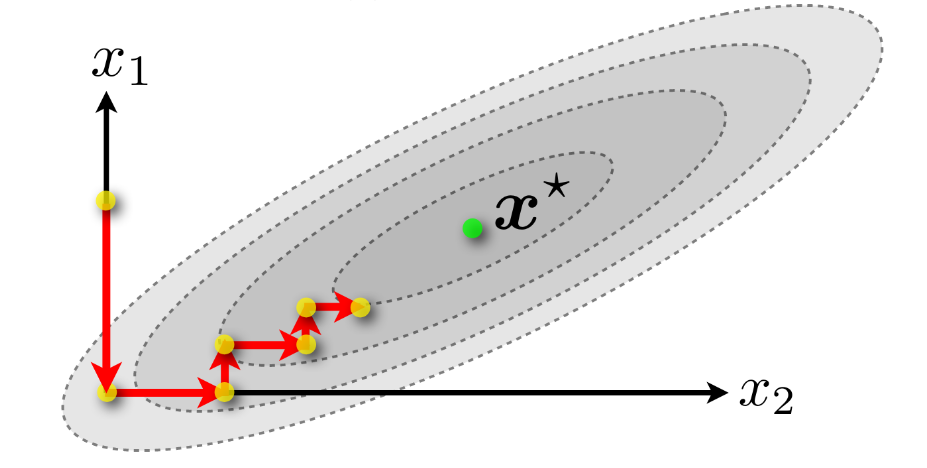
\includegraphics[width=\textwidth,height=\textheight,keepaspectratio]{coordinate_descent}
    % \caption{\label{fig:label} }
  \end{figure}
  \textcolor{blue}{\textbf{Strategy:}} Minimize along one coordinate at a time, while keeping the others fixed.
\end{frame}


\begin{frame}
  \frametitle{Example: Gradient descent}
  \begin{figure}[ht]
    \centering
    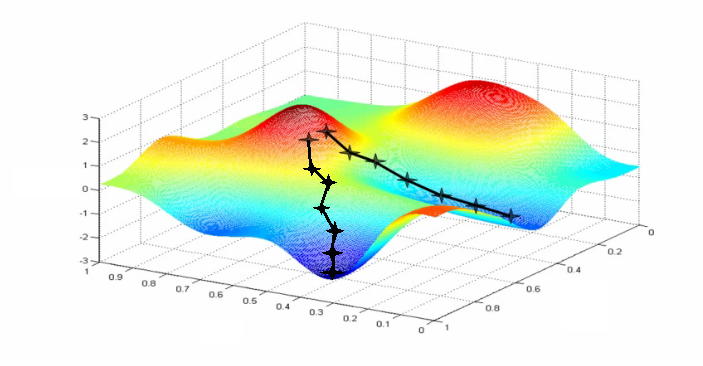
\includegraphics[width=\textwidth,height=\textheight,keepaspectratio]{gradient_descent}
    % \caption{\label{fig:label} }
  \end{figure}
  \textcolor{blue}{\textbf{Strategy:}} Follow the direction of (local) \textbf{steepest descent}.
\end{frame}


\begin{frame}
  \frametitle{}
  \begin{figure}[ht]
    \centering
    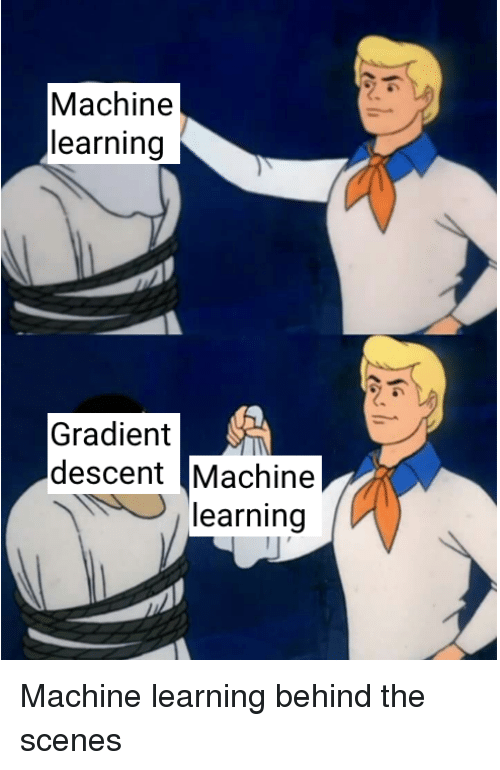
\includegraphics[width=\textwidth,height=\textheight,keepaspectratio]{gradient_descent_meme}
    \caption{\label{fig:label} }
  \end{figure}
\end{frame}

\begin{frame}
  \frametitle{Optimization in other settings}
  \begin{itemize}
    \item \textcolor{blue}{Second order}
          \begin{itemize}
            \item if high precision in solution is required
            \item too \textbf{expensive} in high dimensions
          \end{itemize}
    \item \textcolor{blue}{Zeroth order}
          \begin{itemize}
             \item no gradient or functional representation available
             \item only function values
             \item for simulation, hyperparameters, black box models
          \end{itemize}
    \item constrained problems
    \item discrete optimization
          \begin{itemize}
            \item involving graphs, traveling salesman
            \item scheduling
          \end{itemize}
  \end{itemize}
\end{frame}


\section{Convexity}%
\label{sec:}

\begin{frame}
  \frametitle{Convex sets}
  A set $C$ is \textcolor{blue}{convex} if the line segment between any two points remains inside $C$, i.e.\ for any $x,y \in C$ and $\lambda\in [0,1]$.
  \begin{figure}[ht]
    \centering
    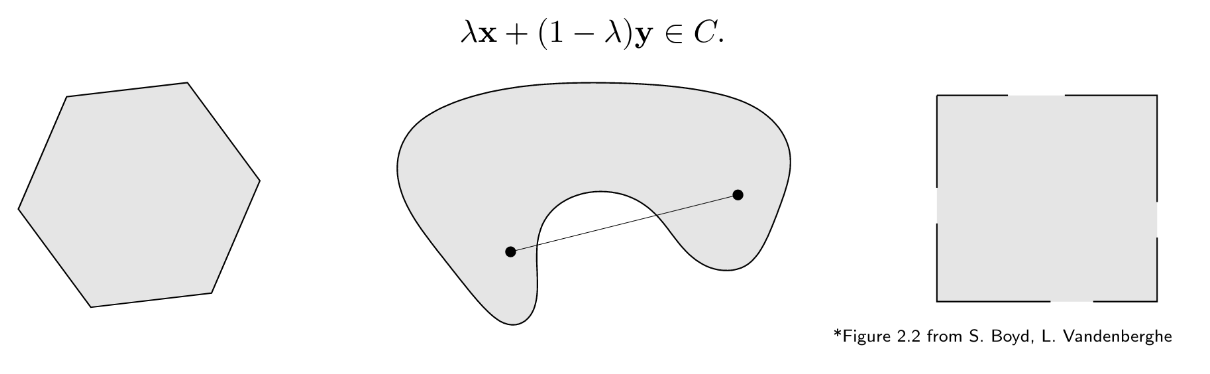
\includegraphics[width=\textwidth,height=\textheight,keepaspectratio]{convex_sets}
    % \caption{\label{} }
  \end{figure}
  \begin{center}
    Which of these sets are convex?
  \end{center}

\end{frame}

\begin{frame}
  \frametitle{Properties of convex sets}
  \begin{itemize}
    \item intersection remains convex
    \item can separated by a hyperplane
    \item projections onto them are unique
          \begin{equation}
            P_C(x) := \argmin_{y\in C} \Vert y-x \Vert
          \end{equation}
  \end{itemize}
\end{frame}


\begin{frame}
  \frametitle{Convex functions}
  We call a function $f \to \R\cup\{+\infty\}$ \textcolor{blue}{convex} if the function values lie below the line segment between $(x, f(x))$ and $(y, f(y))$, i.e./ for any $\lambda\in [0,1]$
  \begin{figure}[ht]
    \centering
    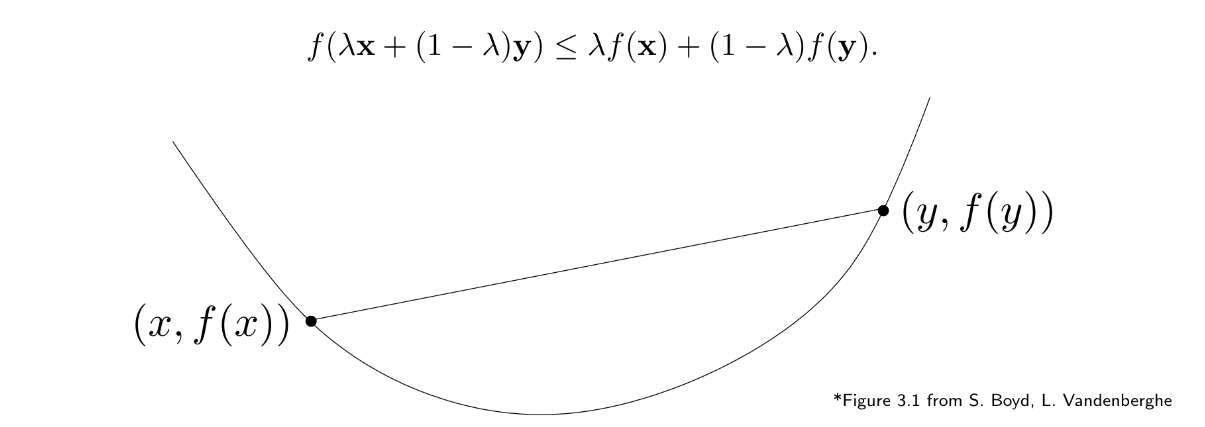
\includegraphics[width=\textwidth,keepaspectratio]{convex_functions}
  \end{figure}

  Sometimes we will call $\{x: f(x)< +\infty \}$ the \textit{domain} of $f$.

\end{frame}


\begin{frame}
  \frametitle{Motivation: Convex optimization}
  Are of the form
  \begin{equation}
    \begin{aligned}
      &\min_x \, f(x) \\
      &\text{such that $x\in C$}
    \end{aligned}
  \end{equation}
  where \textcolor{blue}{both}
  \begin{itemize}
    \item $f$ is a convex function
    \item $C$ is a convex set
  \end{itemize}
  Why?
  \begin{itemize}
    \item \textit{Every local minimum is a global minimum.}
    \item Not all problems are convex but can be used as approximate model.
  \end{itemize}

\end{frame}


\begin{frame}
  \frametitle{Motivation: Provably (efficiently) solving convex problems}
  For convex optimization problems, basically all algorithms
  \begin{itemize}
    \item Coordinate Descent, (Stochastic) Gradient Descent, Proj.\ GD
  \end{itemize}
  \textbf{converge} \textcolor{blue}{provably} to a global optimum including a
  \begin{itemize}
    \item \textbf{quantitative bound}.
  \end{itemize}

  \begin{block}{ Example Theorem }
    Let $f: \R^d \to \R$ be convex then the \textbf{\textcolor{blue}{convergence rate}} is proportional to $1/k$, i.e.\
    \begin{equation}
      f(x_k) - f(x^*) \le \frac{c}{k}
    \end{equation}
  \end{block}
  Explanation: The \textcolor{blue}{approximation error} converges to zero and we know how many iterations are needed to achieve given target.
\end{frame}


\begin{frame}
  \frametitle{Examples of convex functions}
  \begin{itemize}
    \item linear: $f(x) = a^T x$
    \item affine: $f(x) = a^T x + b$
    \item exponential: $f(x) = e^{\alpha x}$
    \item norms, $\Vert \cdot \Vert_1, \Vert \cdot \Vert_2, \Vert \cdot \Vert_\infty$ \hfill \textcolor{purple}{show this}
    \item composition of linear and convex: \\
          for example $f(x)=\Vert Ax-b  \Vert^2$
    \item sum of two convex function $f+g$
  \end{itemize}

\end{frame}


\begin{frame}
  \frametitle{Differentiable function}
  Derivative at a point is the \textcolor{blue}{best linear approximation} of the function at this point.
  \begin{figure}[ht]
    \centering
    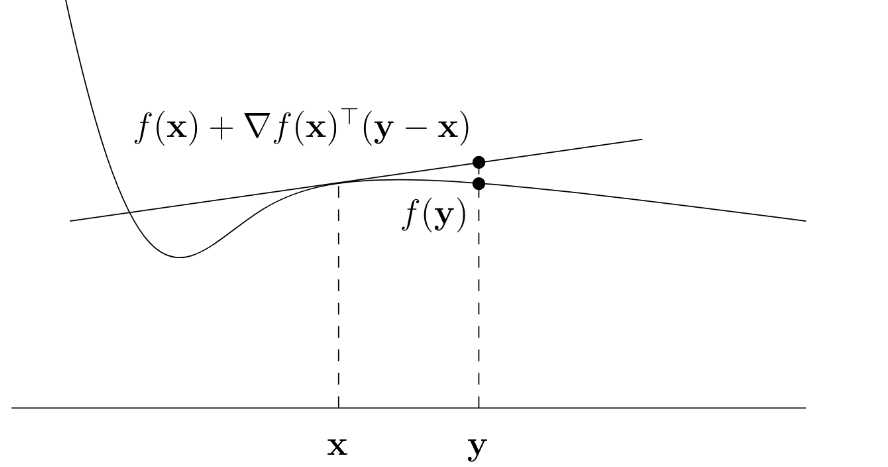
\includegraphics[width=0.8\textwidth,keepaspectratio]{differentiable_function}
    % \caption{\label{fig:label} }
  \end{figure}
  \begin{center}
    Graph of $f(x)+ {\nabla f(x)}^T (y-x)$ is a \textcolor{blue}{tangent hyperplane} to the graph of $f$ at $(x,f(x))$
  \end{center}
\end{frame}


\begin{frame}
  \frametitle{First-order characterization of convexity}

  \begin{figure}[ht]
    \centering
    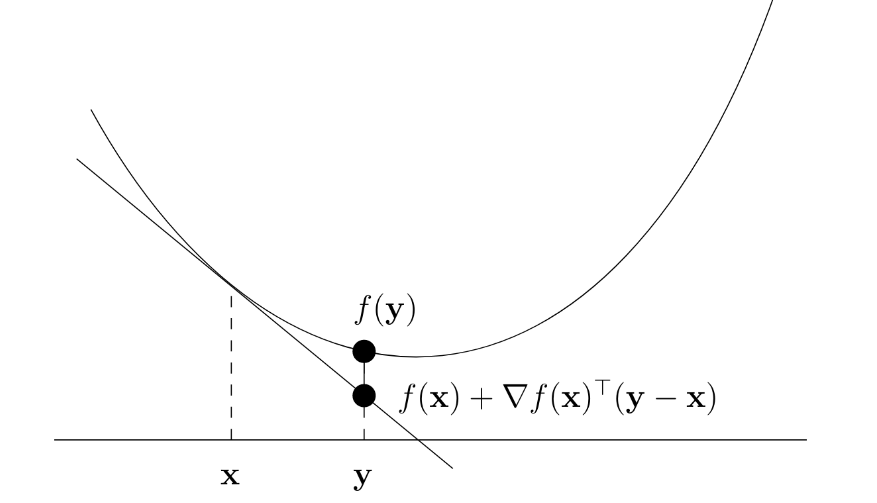
\includegraphics[width=0.8\textwidth,keepaspectratio]{graph_above_tangent}
    % \caption{\label{fig:label} }
  \end{figure}
  If $f$ is differentiable, then
  \begin{center}
    $f$ is convex \emph{if and only if:} $f(y) \ge f(x) + {\nabla f(x)}^T (y-x)$
  \end{center}
\end{frame}


\begin{frame}
  \frametitle{Nonsmooth functions }
  do in fact play a role in practice
  \begin{itemize}
    \item ReLu, Hinge loss, norms
    \item can induce sparsity in the solution
    \item appear as the maximum over a family of functions (max pooling, or min-max)
  \end{itemize}
  \begin{figure}[ht]
    \centering
    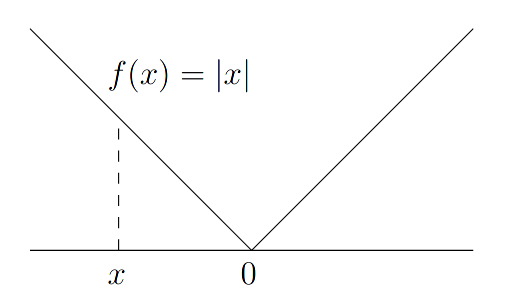
\includegraphics[width=0.7\textwidth,keepaspectratio]{nonsmooth}
    % \caption{\label{fig:label} }
  \end{figure}


\end{frame}

\begin{frame}
  \frametitle{Second-order characterization of convexity}
  If $f$ is \textcolor{blue}{twice differentiable} then it is \textcolor{blue}{convex} \textbf{if and only if} its \emph{Hessian} $\nabla^2 f(x) \in \R^{d \times d}$, given by
  \begin{equation}
    {\nabla^2 f(x)}_{ij} := \frac{\partial^2 f}{\partial x_i \partial x_j}
  \end{equation}
  is \textcolor{blue}{positive semidefinite}, i.e.
  \begin{equation}
    \nabla^2 f(x) \succcurlyeq 0
  \end{equation}

  \textcolor{gray}{A matrix $M$ is \emph{positive semidefinite} if $x^T M x \ge 0$ for all $x$.}\\
  Also used in algorithm like \emph{Newtons} method.

\end{frame}

\begin{frame}
  \frametitle{Examples}
  \begin{itemize}
    \item \textcolor{blue}{quadratic function:} $f(x)= \frac12 x^T Q x + c^T x$, then
          \begin{equation}
            \nabla^2 f(x) = Q
          \end{equation}
          and $f$ is convex iff $Q \succcurlyeq 0$.
    \item \textcolor{blue}{least squares objective:} $f(x) = \Vert Ax -b \Vert^2$, then
          \begin{equation}
             \nabla^2 f(x) = A^T A
          \end{equation}
          is always convex for any A.
  \end{itemize}
\end{frame}


\begin{frame}
  \frametitle{Local minima are global}

  \begin{definition}
    A \textcolor{blue}{local minimum} of $f$ is a point $\bar{x}$ such that there exists $\epsilon>0$
    \begin{equation}
      f(\bar{x}) \le f(y) \quad \forall y: \text{s.t.} \Vert \bar{x}-y \Vert \le \epsilon
    \end{equation}
  \end{definition}

  \begin{lemma}%
    \label{lem:}
    Let $x^*$ be local minimum of a convex function $f$ then $x^*$ is a global minimum.
  \end{lemma}
\textcolor{purple}{Prove this!}
\end{frame}

\begin{frame}
  \frametitle{Local vs. global minima}
  \begin{figure}[ht]
    \centering
    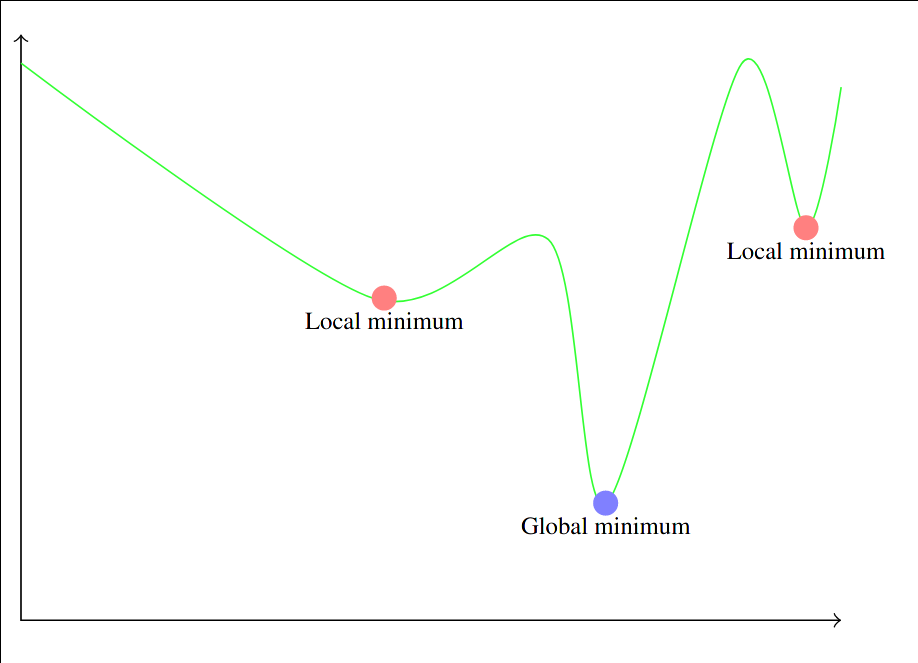
\includegraphics[width=\textwidth,height=\textheight,keepaspectratio]{local_global_minimum}
    % \caption{\label{fig:label} }
  \end{figure}


\end{frame}


\begin{frame}
  \frametitle{Critical points are global minima}

  \begin{definition}
    We call a point $\bar{x}$ \textcolor{blue}{critical} or \textcolor{blue}{stationary} if
    $\nabla f(\bar{x}) = 0$.
  \end{definition}
  \begin{lemma}%
    If $\bar{x}$ is a stationary point of the \textbf{convex} function $f$, then $\bar{x}$ is a \textcolor{blue}{global minimizer} of $f$.
  \end{lemma}
  \textcolor{purple}{Prove this and give a geometric intuition in words using the first order characterization of convexity.}

\end{frame}


\begin{frame}
  \frametitle{Strong convexity}
  \begin{definition}
    We call $f$ \textcolor{blue}{strongly convex} if there exist $\mu> 0$ such that
    \begin{equation}
      f - \frac{\mu}{2} \Vert \cdot \Vert^2 \quad \text{is convex.}
    \end{equation}
  \end{definition}

  Equivalently:
  \begin{itemize}
    \item can be lower bounded by a quadratic
          \begin{equation}
            f(x) + \langle \nabla f(x), y-x \rangle + \frac{\mu}{2} \Vert y-x \Vert^2 \le f(y)
          \end{equation}
    \item Hessian is pos. def. everywhere
          \begin{equation}
            \nabla^2 f(x) \succ 0.
          \end{equation}
  \end{itemize}

\end{frame}

\begin{frame}
  \frametitle{Constrained minimization}

  \begin{minipage}{0.5\textwidth}
    \begin{definition}
      $x^*$ is a minimizer of $f$ \textcolor{blue}{over $C$} if
      \begin{equation}
        f(x^*) \le f(x), \forall x \in C
      \end{equation}
    \end{definition}
    \begin{lemma}%
      $x^*$ is a minimizer of $f$ over $C$ \emph{if and only if}
      \begin{equation}
        \langle \nabla f(x^*), x-x^* \rangle \ge 0 \quad \forall x \in C
      \end{equation}
    \end{lemma}
  % \textcolor{purple}{Prove this.}
  \end{minipage}
  \hfill
  \begin{minipage}{0.45\textwidth}
  \begin{figure}[ht]
    \centering
    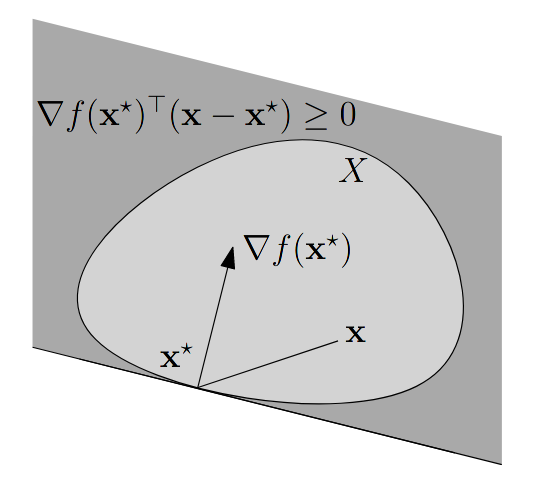
\includegraphics[width=\textwidth,height=\textheight,keepaspectratio]{constrained.png}
    % \caption{\label{fig:label} }
  \end{figure}
  \end{minipage}
\end{frame}

\begin{frame}
  % \frametitle{Proof}
  \begin{lemma}%
    $x^*$ is a minimizer of $f$ over $C$ \emph{if and only if}
    \begin{equation}
      \langle \nabla f(x^*), x-x^* \rangle \ge 0 \quad \forall x \in C
    \end{equation}
  \end{lemma}
  ``$\Leftarrow$'' From the gradient inequality he deduce
  \begin{equation}
    f(x) - f(x^*) \ge \langle \nabla f(x^*), x-x^* \rangle \onslide<2->{\ge 0} \quad \forall x \in C.
  \end{equation}
  ``$\Rightarrow$'' Assume that $f(x^*)\le f(x)$ for all $x \in C$ then $\forall t \in [0, 1]$
  \begin{equation}
    \begin{aligned}
      0 &\le f(x^* + t(x-x^*)) - f(x^*) \\
      0 &\le \lim_{t\to 0} \frac{f(x^* + t(x-x^*)) - f(x^*)}{t} \\
        &= \langle \nabla f(x^*), x-x^* \rangle.
    \end{aligned}
  \end{equation}
  where the last equality follows from the chain rule.\qed

\end{frame}


\begin{frame}
  \frametitle{Existence of a minimizer}

  In general a minimizer \textit{does not need to exist}.
  \begin{itemize}
    \item can be unbounded from below (linear)
    \item bounded but infimum is not obtained
  \end{itemize}
  \begin{center}
    \begin{tikzpicture}
      \draw[->] (-3,0) -- (1.5,0) node[right] {$x$};
      \draw[->] (0,-0.5) -- (0,2.5) node[above] {$y$};
      \draw (0,1) node[right] {$y=1$};
      \draw (1,2.7) node[right] {$f(x)=e^x$};
      \draw[scale=1,domain=-3:1,smooth,variable=\x,blue] plot ({\x}, {exp(\x)});
    \end{tikzpicture}
  \end{center}

  Typically we only consider problems where we assume a minimizer to exist (otherwise our model might be bad).

  \begin{itemize}
    \item if function is strongly convex a minimizer \textit{always} exists.
  \end{itemize}

\end{frame}

\end{document}
